\documentclass{beamer}

% importations de packages utiles
\usepackage[utf8]{inputenc}  % pouvoir écrire avec des accents
\usepackage[french]{babel}  % francophopnie
\usepackage{hyperref}  % liens clicables dans pdf final
\usepackage{tikz}  % pouvoir tracer des dessins sympas
\usetheme{Boadilla}  % thème de beamer
\usepackage{listingsutf8}  % rendu de "code" (avec config ci-dessous)
\definecolor{lstcolor}{rgb}{0.9,0.95,0.95}
\definecolor{lstcommentcolor}{rgb}{0.,0.2,0.}
\lstset{
  frameround=tttt,
  %autogobble,
  frame=single,
  backgroundcolor=\color{lstcolor},
  % extendedchars=true,
  % basicstyle=\ttfamily\small,
  keywordstyle=\bfseries\color{blue},
  identifierstyle=\bfseries\color{red},
  stringstyle=\bfseries\color{orange},
  commentstyle=\color{lstcommentcolor},
  language=Python,
  keepspaces=True,
  basicstyle=\fontfamily{pcr}\selectfont\small, % monospace it for copypasting
  upquote=true,
  columns=flexible,
  showstringspaces=False,
  literate={é}{{\'e}}1
}
\title{La Concurrence}
\subtitle{Concepts de Langages de Programmation}
\author{Juan-Carlos Barros et Daniel Kessler}
% et c'est parti
\begin{document}
\begin{frame}
  \titlepage
\end{frame}

\begin{frame}
  \tableofcontents
\end{frame}

\section{Introduction}
\begin{frame}
  \frametitle{Introduction: la concurrence en-dehors de l'informatique}
  \begin{itemize}
  \item le cerveau est intrinsèquement parallèle
   \begin{itemize}
   \item traitement du stimuli visuel
   \item traitement du stimuli auditif
   \item traitement de la syntaxe
   \item découverte de la sémantique
   \item analyse du sens
   \item comparaison avec les connaissances mémorisées
   \item critique
  \end{itemize}
  % \item les rails
  \item Un processeur est intrinsèquement séquentiel
   \begin{itemize}
   \item exécute une instruction à la fois
   \item premiers ordinateurs: un seul programme à la fois
   \item Plusieurs raisons pour développer parallélisme, concurrence
   \item interruptions pour gérer les I/O, l'horloge, etc.
   \item pouvoir exécuter plusieurs programmes "simultanément"
   \item multiplication des coeurs dans les processeurs
   \item Comment gérer la concurrence dans un processeur?
  \end{itemize}

  \item \ldots
  \end{itemize}
\end{frame}

\section{Les fondamentaux de la concurrence}
\begin{frame}
  \frametitle{Fondamentaux de la concurrence en informatique}
  \begin{itemize}
  \item Situations en informatique où la concurrence est inévitable
  \item Threads vs Processus
  \item Synchrone vs Asynchrone
  \item Problèmes classiques
  \item Solutions classiques
  \end{itemize}
\end{frame}
\begin{frame}
  \frametitle{Situations en informatique où la concurrence est inévitable}
  \begin{itemize}
  \item Le Système d'Exploitation
  \item Toute application distribuée (par exemple un service web)
  \end{itemize}
\end{frame}
\begin{frame}
  \frametitle{Threads vs Processus}
  \begin{itemize}
  \item Processus: idéal pour déléguer des calculs intensifs
  \item Threads: idéal pour déléguer des opérations I/O
  \end{itemize}
\end{frame}
\begin{frame}
  \frametitle{Communication synchrone vs asynchrone}
  \begin{itemize}
  \item synchrone: \ldots
  \item asynchrone: \ldots
  \end{itemize}
\end{frame}
\begin{frame}
  \frametitle{Problèmes classiques}
  \begin{itemize}
  \item ``race condition''
  \item famine (starvation)
  \item interblocage (deadlock)
  \item $\rightarrow$ sections critiques
  \end{itemize}
  $\rightarrow$ ``jeu de Dekker'' pour illustrer 
\end{frame}
\begin{frame}
  \frametitle{Solutions classiques}
  \begin{itemize}
  \item Verrous
  \item Sémaphores de Dijkstra
  \item Moniteurs
  \item Futures/Promises
  \end{itemize}
\end{frame}
\begin{frame}
  \frametitle{Solutions classiques}
  Le langage de modélisation graphique \textbf{UML} se prête bien à décrire ce
  genre d'outil.
  \par
  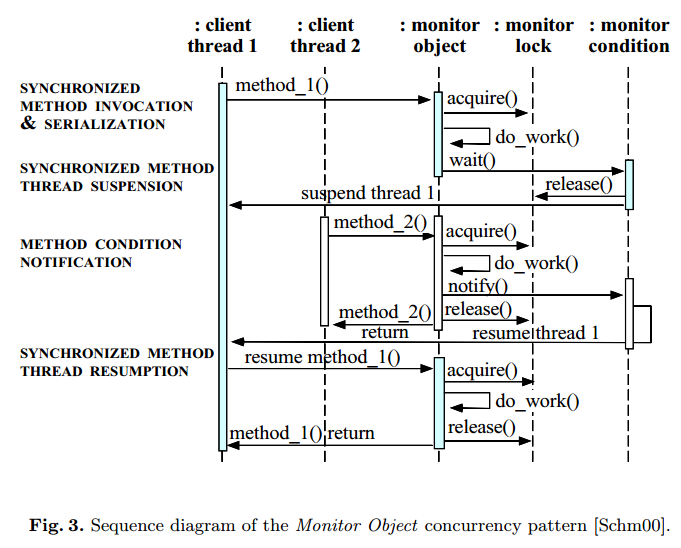
\includegraphics[width=.7\textwidth]{monitor.png}
\end{frame}
\begin{frame}
  \frametitle{Exemple d'implémentation}
  (code Python ou Java)
\end{frame}

\section{Modèle d'Acteurs de Hewitt}
\begin{frame}
  \frametitle{Éviter la mémoire partagée?}
  \begin{itemize}
  \item La mémoire partagée est la source de la plupart des problèmes
  \item Les communications ne devraient se faire que par des \textbf{immuables}
  \end{itemize}
\end{frame}
\begin{frame}[fragile]
  \frametitle{Modèle d'Acteurs de Hewitt}
  Un \textbf{acteur} peut:
  \begin{itemize}
  \item Envoyer des \textbf{messages} à d'autres acteurs
  \item Créer d'autres acteurs
  \item Décider de son comportement à la prochaine réception de message
  \end{itemize}
\end{frame}
\begin{frame}[fragile]
  \frametitle{Modèle d'Acteurs de Hewitt}
  Le langage \textbf{Erlang} exploite bien ce modèle.
  \begin{center}
\begin{lstlisting}[language=erlang]
-module(acteur).
-export([start/0, machin/0]).

machin() ->
    receive
        hello ->
            io:format("Machin dit bonjour.~n", [])
    end.

start() ->
    Machin_PID = spawn(acteur, machin, []),
    Machin_PID ! hello.
\end{lstlisting}
\end{center}
  Plus récemment, le langage \textbf{Scala} utilise ce même modèle, à travers le
  ``toolkit'' \textbf{Akka}.
\end{frame}
\begin{frame}
  \frametitle{Modèle d'Acteurs de Hewitt}
  Le modèle d'acteurs a influencé le \textbf{$\pi$-calculus} (algèbre de processus)
  \par\bigskip
  \begin{quotation}\small
    Now, the pure $\lambda$-calculus is built with just two kinds of thing: terms
    and variables. Can we achieve the same economy for a process calculus? Carl
    Hewitt, with his actors model, responded to this challenge long ago; he
    declared that a value, an operator on values, and a process should all be
    the same kind of thing: an actor.

    (\ldots)
    
    So, in the spirit of Hewitt, our first step is to demand that all things
    denoted by terms or accessed by names—values, registers, operators,
    processes, objects—are all of the same kind of thing; they should all be
    processes.
  \end{quotation}
  \hfill Robin Milner, inventeur du $\pi$-calculus (\textit{Turing Lecture} 1993)
\end{frame}
\begin{frame}[fragile]
  \frametitle{Modèle d'Acteurs de Hewitt}
  Lauer et Needham on montré en 1978 que les modèles de concurrence basé sur
  processus et les modèles basés sur messages sont équivalents (``duaux'').
  \par\bigskip
  \hfill{$\rightarrow$ \footnotesize{}cf. \textit{On the duality of operating system structures}
    H. Lauer, R. Needham 1978}
\end{frame}

\section{Autres approches}
\begin{frame}
  \frametitle{Autres approches}
  \begin{itemize}
  \item{Programmation événementielle} 
  \begin{itemize}
  \item utile pour les GUIs, mais difficile à analyser
  \item ``event loop''
  \item ``event handlers'' (callbacks)
  \end{itemize}
  
  \item{Transactions }
  \begin{itemize}
  \item idée inspirée des Bases de Donnée
  \item rendre ``atomique'' la section critique
  \item idée exploitée par exemple dans le langage \textbf{Clojure}
  \end{itemize}
  
  \item{Coroutines}
  \begin{itemize}
  \item coroutines: des routines concurrentes pouvant ``vivre'' dans le même thread
  \item idée exploitée par exemple dans le langage \textbf{Go} (``goroutines'')
  \end{itemize}

  \item{Réseaux de Petri} (pour la modélisation)
  \end{itemize}
\end{frame}

\section{Conclusion}
\begin{frame}
  \frametitle{Conclusion: au-delà de la concurrence}
  Réseaux de neurone!
\end{frame}


\end{document}